% !TEX root =  main.tex
\chapter{Experimental Evaluation}
\label{chap:experiments}
\pagestyle{plain}

% Path to generated graphs
\graphicspath{{graphs/}}

This chapter presents the experimental evaluation of the complete pipeline. We first describe the experimental setup, including the dataset, system environment, and hyperparameter configuration. We then analyze the quality of the generated query workload and evaluate the active learning process together with the accuracy of the trained cardinality estimator. All figures in this chapter are generated automatically by the evaluation module of the pipeline, providing an accurate and reproducible representation of the system's behavior on real data.


\section{Experimental Setup}

All experiments are conducted on the Internet Movie Database (IMDB), a widely used benchmark in learned cardinality estimation research~\cite{DBLP:conf/cidr/KipfKRLBK19}. The IMDB dataset consists of four core tables: \texttt{title\_basics} containing metadata for approximately 10 million titles including title type, production year, runtime, and genre information; \texttt{name\_basics} containing metadata for approximately 12 million people associated with titles; \texttt{title\_principals} serving as a junction table linking titles to the principal cast and crew with approximately 56 million records; and \texttt{title\_ratings} containing user ratings and vote counts for approximately 1.3 million titles. The schema defines foreign key relationships between tables through the \texttt{tconst} and \texttt{nconst} identifiers, enabling meaningful join queries. Figure~\ref{fig:imdb_schema} illustrates the schema relationships.

\begin{figure}[tb]
\centering
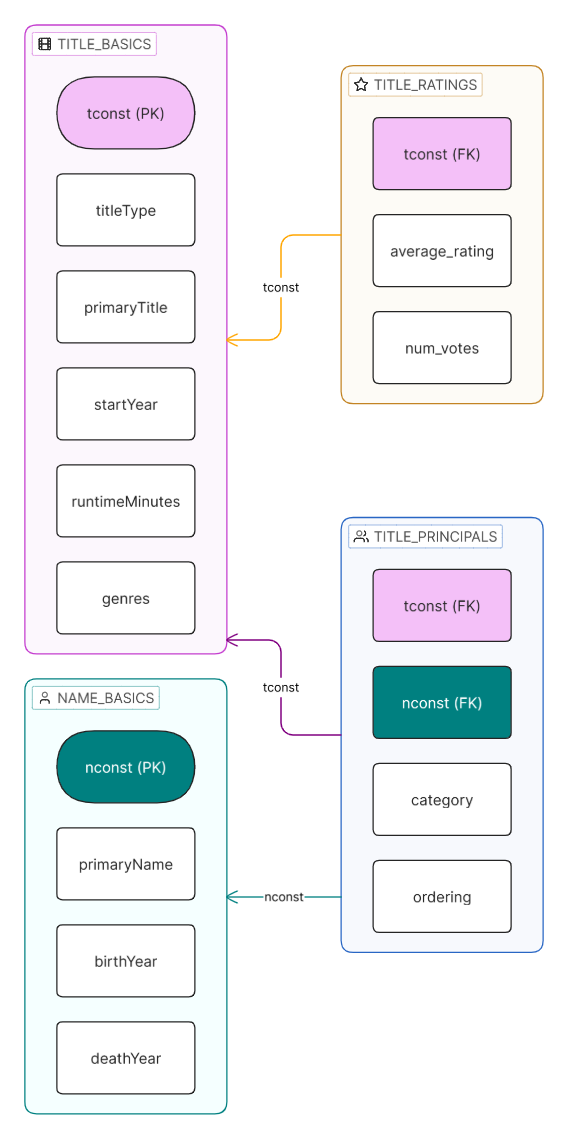
\includegraphics[width=\textwidth,height=0.75\textheight,keepaspectratio]{Report/graphs/imdb_er.png}
\caption{Entity-relationship diagram of the IMDB database schema. The \texttt{title\_principals} table acts as a central junction connecting titles to people, while \texttt{title\_ratings} provides aggregate user feedback per title. These relationships define the valid join paths for generated queries.}
\label{fig:imdb_schema}
\end{figure}

Table~\ref{tab:exp_config} summarizes the configuration parameters used across all experiments. These values were selected based on preliminary experiments and align with recommended settings from the MSCN literature. The pipeline is implemented in Python using PyTorch for the neural network training. PostgreSQL serves as the database backend, and Ollama provides local LLM hosting. All experiments are executed on a standard workstation.

\begin{table}[tb]
\centering
\caption{Experimental configuration parameters.}
\label{tab:exp_config}
\begin{tabular}{|l|l|c|}
\hline
\textbf{Category} & \textbf{Parameter} & \textbf{Value} \\
\hline
\multirow{3}{*}{Query Generation} & Total queries & 5000 \\
 & LLM batch size & 20 \\
 & LLM model & Llama 3.2 \\
\hline
\multirow{2}{*}{Database} & Materialized samples & 1000 \\
 & Max retries & 2 \\
\hline
\multirow{4}{*}{Active Learning} & Strategy & random / uncertainty / mc\_dropout \\
 & Rounds & 5 \\
 & Acquisition batch size & 200 \\
 & MC Dropout passes ($T$) & 25 \\
\hline
\multirow{4}{*}{MSCN Training} & Hidden units & 256 \\
 & Learning rate & $10^{-4}$ \\
 & Epochs per round & 10 \\
 & Training batch size & 1024 \\
\hline
\end{tabular}
\end{table}

\section{Query Generation Analysis}

The quality of the generated query workload is a critical factor in training an effective estimator. Figure~\ref{fig:structural_analysis} shows the combined distribution of tables, joins, and predicates across all generated queries. The distributions reveal a balanced mix of single-table, two-table, and three-table queries, ensuring that the model is trained on queries of varying structural complexity. The predicate count distribution demonstrates that most queries include between one and three filter conditions, reflecting realistic workload patterns.

\begin{figure}[tb]
\centering

\includegraphics[width=\textwidth]{data_structural_features.png}
\caption{Structural feature distributions across the generated workload. The balanced coverage of different table counts, join complexities, and predicate counts confirms that the diversity hint mechanism prevents the LLM from converging on a narrow subset of query patterns.}
\label{fig:structural_analysis}
\end{figure}

Figure~\ref{fig:validation_results} shows the query validation success rate across the four validation layers. The high pass rate demonstrates that the prompt engineering strategy effectively guides the LLM to produce well-formed, schema-compatible queries, with only a small fraction rejected at each validation stage.

\begin{figure}[tb]
\centering

\includegraphics[width=0.85\textwidth]{data_query_validation.png}
\caption{Query validation success rates across the four filtering layers. The high pass rate at each stage demonstrates the effectiveness of the prompt engineering constraints in guiding the LLM toward valid query structures.}
\label{fig:validation_results}
\end{figure}

Figure~\ref{fig:detail_distributions} provides a closer look at the individual distributions of tables and predicates per query, while Figure~\ref{fig:joins_distribution} shows the join condition distribution separately.

\begin{figure}[tb]
\centering
\begin{minipage}[t]{0.48\textwidth}
\centering

\includegraphics[width=\textwidth]{data_tables_distribution.png}
\caption{Distribution of table count per query. The weighted mix of single-table, two-table, and three-table queries ensures coverage of both simple selections and complex multi-way joins.}
\label{fig:tables_distribution}
\end{minipage}
\hfill
\begin{minipage}[t]{0.48\textwidth}
\centering

\includegraphics[width=\textwidth]{data_predicates_distribution.png}
\caption{Distribution of predicate count per query. The majority of queries contain one to three predicates, reflecting a realistic range of filter complexities.}
\label{fig:predicates_distribution}
\end{minipage}
\end{figure}

\begin{figure}[tb]
\centering

\includegraphics[width=0.85\textwidth]{data_joins_distribution.png}
\caption{Distribution of join conditions per query. Queries with zero joins correspond to single-table queries, while one and two join conditions correspond to two-table and three-table queries, respectively.}
\label{fig:joins_distribution}
\end{figure}

Figure~\ref{fig:cardinality_dist} shows the distribution of true cardinalities for the labeled queries on a logarithmic scale. The distribution spans from single-digit cardinalities to tens of millions of rows, which is essential for training a model that generalizes across the full selectivity spectrum. Without this range, the model would be unable to distinguish between highly selective filters and broad scans.

\begin{figure}[tb]
\centering
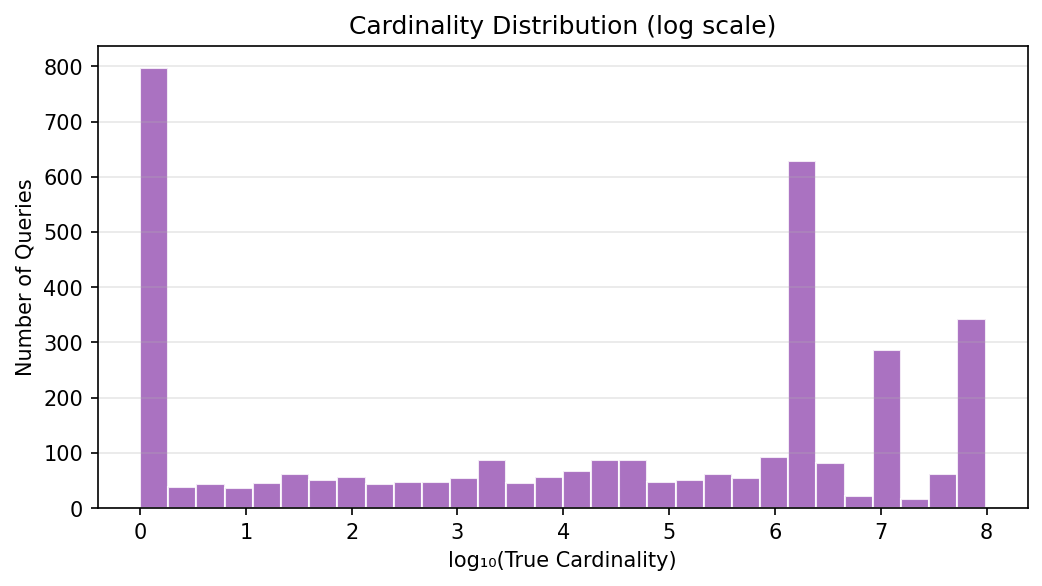
\includegraphics[width=0.85\textwidth]{data_cardinality_distribution.png}
\caption{Distribution of true cardinalities ($\log_{10}$ scale). The wide range spanning several orders of magnitude forces the model to learn accurate estimates for both highly selective queries returning few rows and broad queries spanning millions of tuples.}
\label{fig:cardinality_dist}
\end{figure}


From a broader perspective, the structural properties of the generated workload can be understood through a set of complementary distributions. Figure~8.2 provides a consolidated view of three orthogonal dimensions—tables, joins, and predicates—offering a compact justification that the generated corpus is structurally diverse rather than biased toward a single query template. This diversity is essential, as it ensures that the downstream model is exposed to heterogeneous query patterns, which in turn enables active learning to identify and prioritize informative samples from a varied pool.

Figures~8.4-8.6 further decompose these dimensions to provide more detailed insights. Figure~8.4 illustrates the distribution of table counts per query, which serves as a proxy for query graph size. The presence of both single-table and multi-table queries indicates that the workload spans low-dimensional as well as higher-dimensional join spaces, allowing the model to learn how estimation complexity increases with relational context. Figure~8.5 captures the predicate count distribution, reflecting variations in filtering complexity. Queries with fewer predicates tend to produce broader result sets, whereas those with multiple predicates correspond to more selective conditions. This spread across selectivity regimes confirms that the workload is not trivially homogeneous and challenges the model across a range of filtering scenarios. Complementing this, Figure~8.6 presents the distribution of join counts, highlighting the structural complexity of the workload. A balanced presence of queries with zero, one, and multiple joins demonstrates that the model is exposed to both base-table selectivity patterns and the additional uncertainty introduced by join operations.

Finally, Figure~8.7 examines the distribution of true cardinalities on a logarithmic scale. The observed spread across several orders of magnitude reflects the inherently skewed nature of cardinality estimation tasks. This long-tailed distribution is particularly important, as it ensures that the model is trained on both highly selective queries and large-scale scans. Such diversity in target values justifies the use of relative error metrics, such as Q-error, which are better suited for evaluating performance across varying cardinality scales.

Taken together, these analyses demonstrate that the generated workload captures a wide range of structural and statistical characteristics. This diversity forms the foundation for effective model training and provides the necessary conditions for active learning to operate efficiently, ultimately improving both generalization and robustness of the learned estimator.

\section{Active Learning and Model Training Results}

This section presents the results from the active learning loop, examining how the model's accuracy evolves across rounds and how effectively it learns to predict query cardinalities.

Figure~\ref{fig:learning_curves_comparison} shows the active learning curve, plotting the validation median Q-error against the number of labeled training queries. The decreasing trend confirms that the model benefits from each active learning round, achieving progressively lower estimation errors as the training set grows with informatively selected queries.

\begin{figure}[tb]
\centering

\includegraphics[width=0.9\textwidth]{train_learning_curve_random.png}
\caption{Active learning curve showing validation median Q-error versus the number of labeled queries. The steep initial decline demonstrates rapid learning from the first few rounds, while the flattening tail indicates diminishing returns as the model approaches its capacity on the given data.}
\label{fig:learning_curves_comparison}
\end{figure}


Figure~\ref{fig:training_loss_rounds} shows how the training loss evolves across active learning rounds. Each subsequent round starts from a lower loss baseline, confirming that the model retains useful representations from earlier rounds while benefiting from the newly acquired training data.

\begin{figure}[tb]
\centering
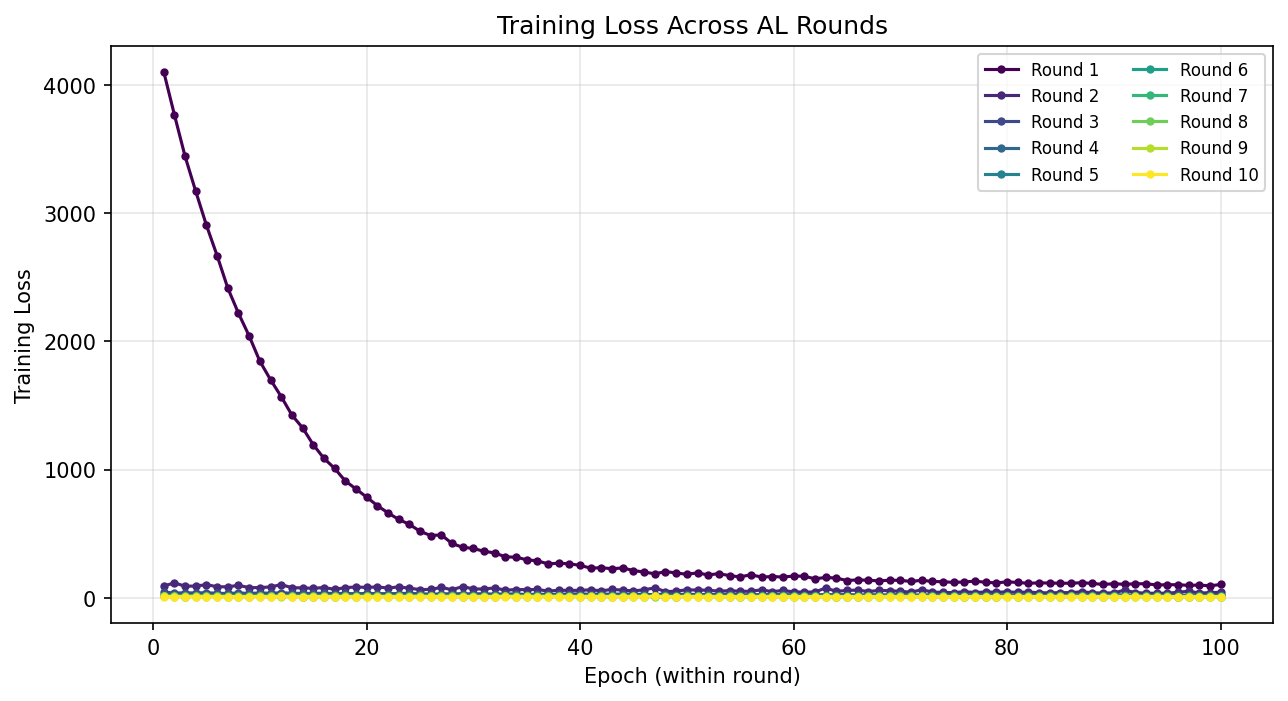
\includegraphics[width=0.9\textwidth]{train_loss_curve.png}
\caption{Training loss curves across active learning rounds. The consistently decreasing trajectory demonstrates stable convergence, with each round starting from a better baseline than the previous one due to the expanded and more informative training set.}
\label{fig:training_loss_rounds}
\end{figure}


Figure~\ref{fig:pred_vs_actual} presents a scatter plot of predicted versus actual cardinalities on a log-log scale. Points near the diagonal line $y = x$ indicate accurate predictions, while deviations reveal systematic estimation biases. The tight clustering around the diagonal across several orders of magnitude demonstrates that the trained model achieves good calibration for both small and large cardinalities.

\begin{figure}[tb]
\centering
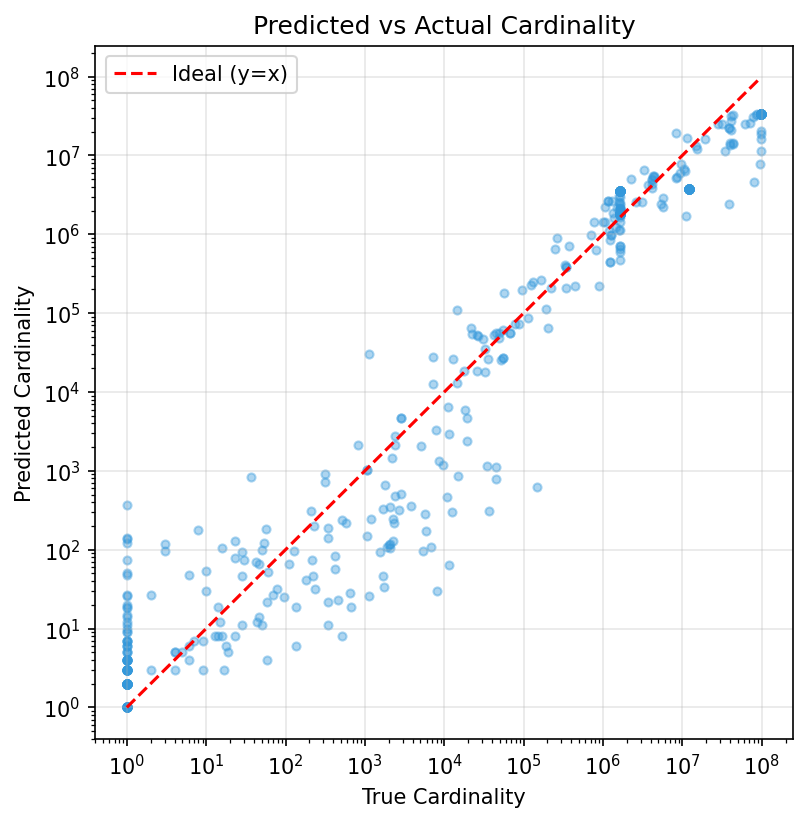
\includegraphics[width=0.85\textwidth]{test_predicted_vs_actual.png}
\caption{Predicted vs.\ actual cardinality on a log-log scale. The concentration of points along the diagonal indicates that the MSCN model produces well-calibrated estimates across the full cardinality range, from selective single-table queries to large multi-table joins.}
\label{fig:pred_vs_actual}
\end{figure}


Figures~\ref{fig:qerror_cdf} and~\ref{fig:qerror_boxplot} provide complementary perspectives on the Q-error distribution. The CDF reveals the proportion of queries falling below each error threshold, showing that the majority of predictions are within a small factor of the true cardinality. The per-round box plots illustrate how the error distribution tightens with each active learning round, confirming the progressive improvement in estimation quality.

\begin{figure}[tb]
\centering
\begin{minipage}[t]{0.48\textwidth}
\centering
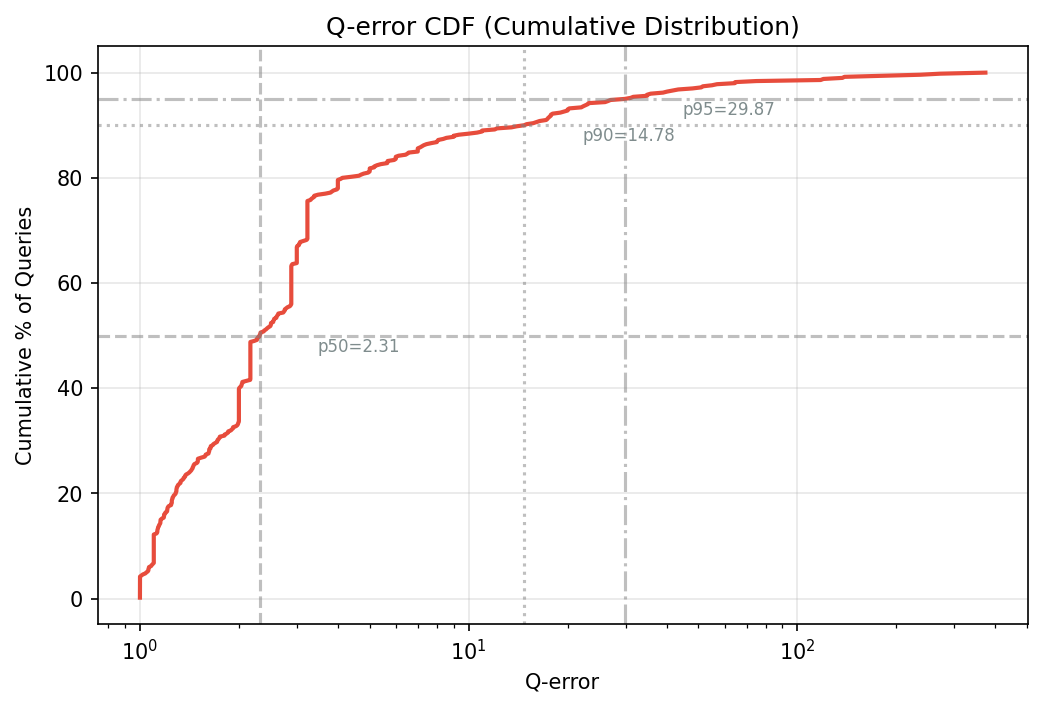
\includegraphics[width=\textwidth]{test_qerror_cdf.png}
\caption{Cumulative distribution function of Q-errors. The steep rise at low Q-error values indicates that the majority of queries are estimated within a factor of 2-5 of their true cardinality.}
\label{fig:qerror_cdf}
\end{minipage}
\hfill
\begin{minipage}[t]{0.48\textwidth}
\centering
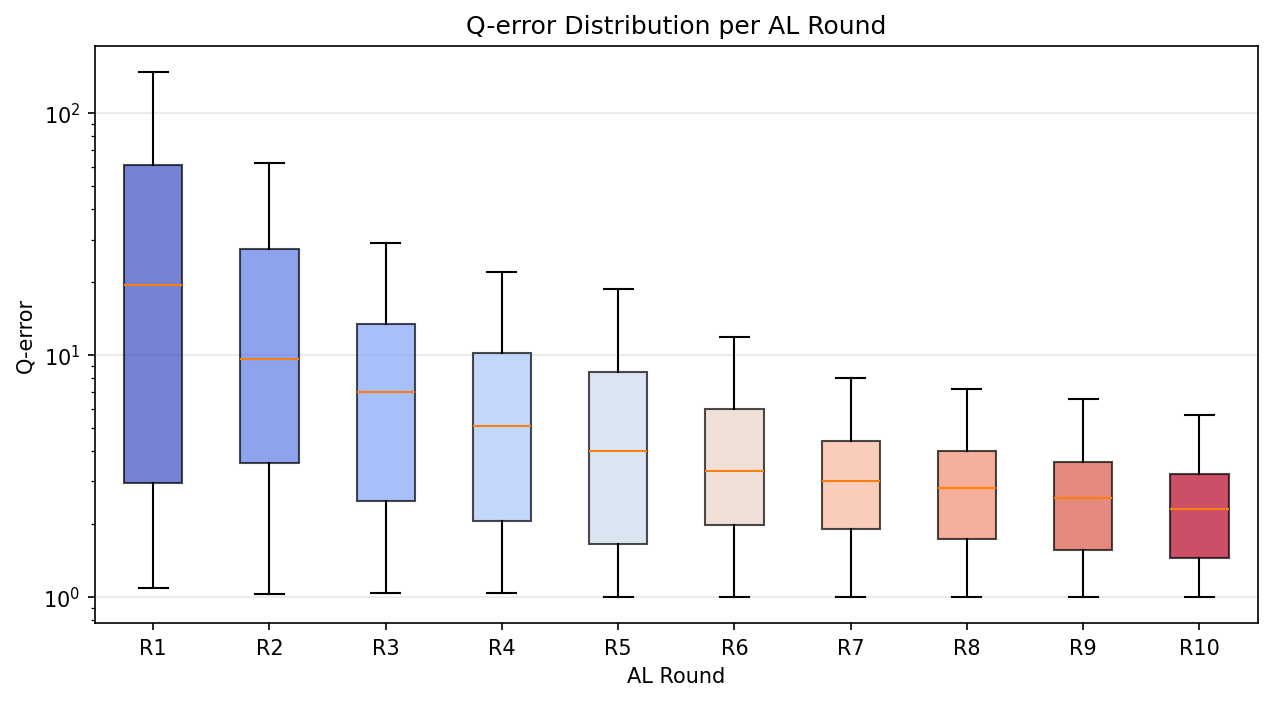
\includegraphics[width=\textwidth]{test_qerror_per_round.png}
\caption{Q-error box plots per active learning round. The narrowing boxes and decreasing medians demonstrate how each round improves estimation accuracy.}
\label{fig:qerror_boxplot}
\end{minipage}
\end{figure}


Figure~\ref{fig:qerror_stats} provides a detailed statistical view of Q-error metrics across active learning rounds, showing the median, mean, 90th percentile, and 95th percentile values.

\begin{figure}[tb]
\centering
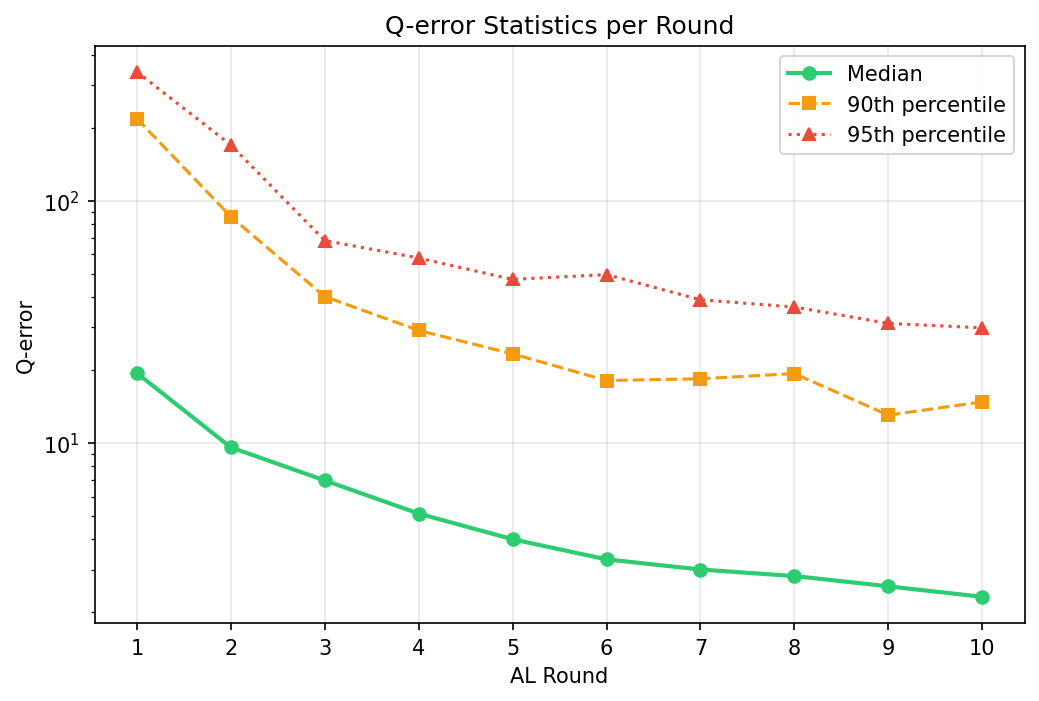
\includegraphics[width=0.9\textwidth]{test_qerror_stats.png}
\caption{Q-error statistics across active learning rounds. The consistent decrease in all percentile metrics confirms that active query selection improves not only typical-case accuracy but also tail-end performance on the most challenging queries.}
\label{fig:qerror_stats}
\end{figure}


From a broader perspective, the behavior of the model across training and evaluation can be interpreted through a combination of complementary metrics. Figure~8.8 captures the overall learning trajectory by plotting the validation median Q-error against the number of labeled queries under a random acquisition strategy. The consistent decrease in median Q-error indicates that increasing the supervision budget leads to improved estimation accuracy. More importantly, the relative reduction in median Q-error from the initial to the final round quantifies the practical benefit obtained per unit of labeling effort, highlighting the efficiency of the training process.

Figure~8.9 provides insight into the optimization dynamics within each active learning round. The steep decline in training loss during early epochs demonstrates that the model is able to effectively fit the available labeled data, while the gradual flattening in later stages indicates convergence. The fact that subsequent rounds begin from lower loss baselines suggests that the model retains useful representations and continues to benefit from newly added samples. This behavior confirms both the stability of the training process and the continued informativeness of the selected queries.

The quality of the learned estimator is further illustrated in Figure~8.10, which compares predicted and actual cardinalities on a log-log scale. The close alignment of points along the diagonal indicates accurate predictions across multiple orders of magnitude, while deviations from this line reveal regions of systematic bias. In particular, increased dispersion at the extremes of the distribution highlights the inherent difficulty of estimating very small or very large cardinalities, which is consistent with the known challenges of long-tailed data distributions.

Figures~8.11 and~8.12 provide complementary views of estimation error using Q-error metrics. The cumulative distribution function in Figure~8.11 shows the proportion of queries achieving Q-error below a given threshold, enabling direct and interpretable quality assessments. For instance, percentile markers such as p50, p90, and p95 summarize typical and worst-case performance, aligning with standard evaluation practices in database systems research. Meanwhile, the per-round box plots in Figure~8.12 illustrate how the full error distribution evolves during active learning. The progressive reduction in median values, along with the shrinking interquartile range and lower upper whiskers, indicates not only improved average accuracy but also enhanced robustness, with fewer extreme estimation errors over time.

Taken together, these results demonstrate that the proposed training pipeline yields a well-calibrated and robust cardinality estimator. The combination of improving learning curves, stable optimization behavior, accurate calibration, and tightening error distributions provides strong evidence that the model benefits systematically from additional labeled data while maintaining generalization across diverse query patterns.

\section{Labeling Efficiency Analysis}

A central claim of this thesis is that active learning reduces the number of expensive database executions needed to train an accurate model. Figure~\ref{fig:labeling_efficiency} directly visualizes this by comparing the labeling effort of the active learning approach against a fully supervised baseline. The results show that the active learning pipeline achieves comparable model accuracy while labeling only a fraction of the total query pool.

\begin{figure}[tb]
\centering
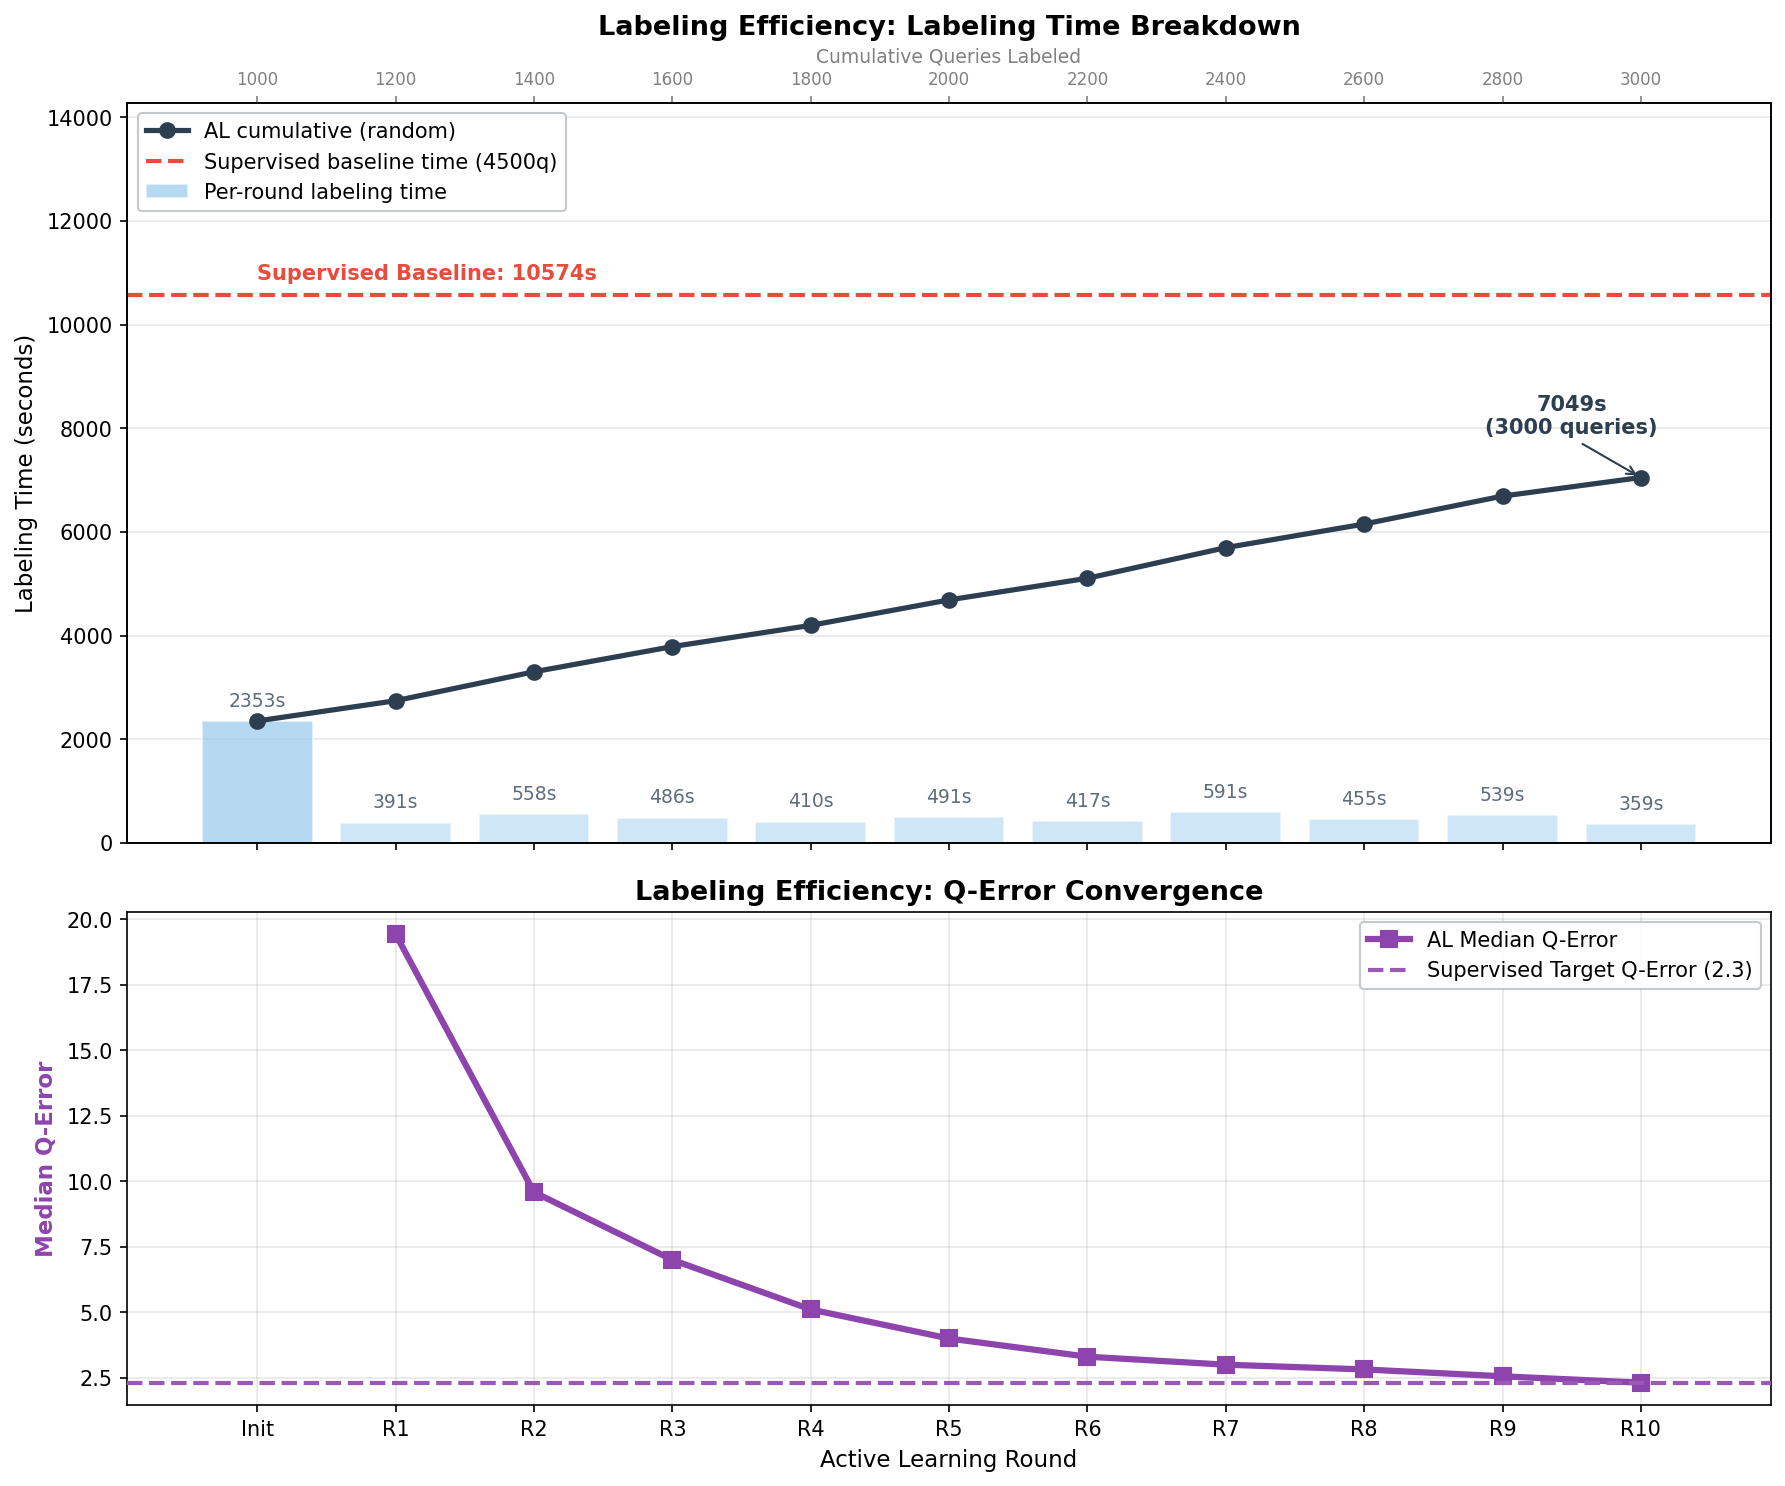
\includegraphics[width=\textwidth]{analysis_labeling_efficiency.png}
\caption{Labeling efficiency comparison. The active learning approach achieves competitive accuracy with significantly fewer labeled queries than a fully supervised baseline, demonstrating that intelligent query selection reduces the dominant cost factor in the pipeline.}
\label{fig:labeling_efficiency}
\end{figure}

Figure~\ref{fig:labeling_rate} shows the labeling success rate across the pipeline, indicating what fraction of queries were successfully labeled within the timeout constraints.

\begin{figure}[tb]
\centering
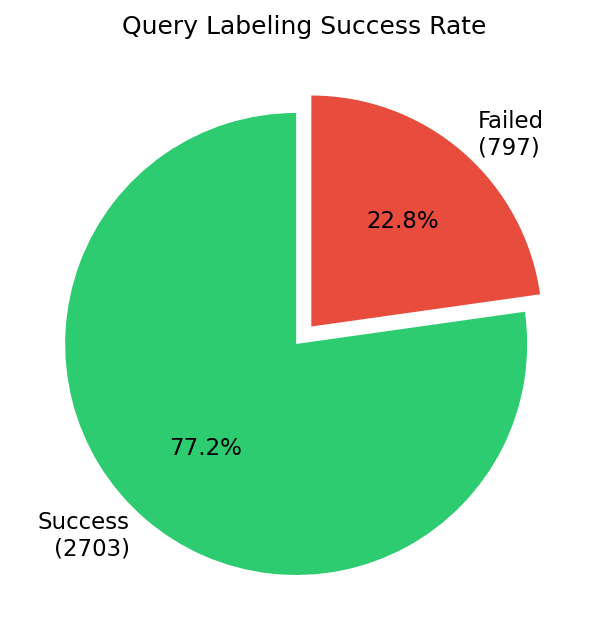
\includegraphics[width=0.85\textwidth]{analysis_labeling_rate.png}
\caption{Labeling success rate across the pipeline. Queries that exceed
the database timeout or fail after repeated retries are excluded from the final
labeled workload. The high success rate confirms that the generated queries are
overwhelmingly executable within the configured time limits.}
\label{fig:labeling_rate}
\end{figure}

\section{Comparison with PostgreSQL Optimizer}

To contextualize the MSCN model's accuracy, we compare its cardinality estimates directly against those produced by the PostgreSQL native query optimizer. Figures~\ref{fig:pg_cdf} and~\ref{fig:pg_scatter} present this comparison using the same validation queries.

\begin{figure}[tb]
\centering
\begin{minipage}[t]{0.48\textwidth}
\centering

\includegraphics[width=\textwidth]{compare_pg_vs_mscn_cdf.png}
\caption{Q-error CDF comparing the MSCN model against PostgreSQL's native estimator. A curve shifted further left indicates better estimation accuracy.}
\label{fig:pg_cdf}
\end{minipage}
\hfill
\begin{minipage}[t]{0.48\textwidth}
\centering

\includegraphics[width=\textwidth]{compare_pg_vs_mscn_scatter.png}
\caption{Predicted vs.\ actual scatter comparing MSCN and PostgreSQL. Points closer to the diagonal represent more accurate estimates.}
\label{fig:pg_scatter}
\end{minipage}
\end{figure}

\section{Discussion}

Figure~\ref{fig:pipeline_summary} shows the full pipeline dashboard, pulling together the key numbers from every stage into one view.

\begin{figure}[tb]
\centering
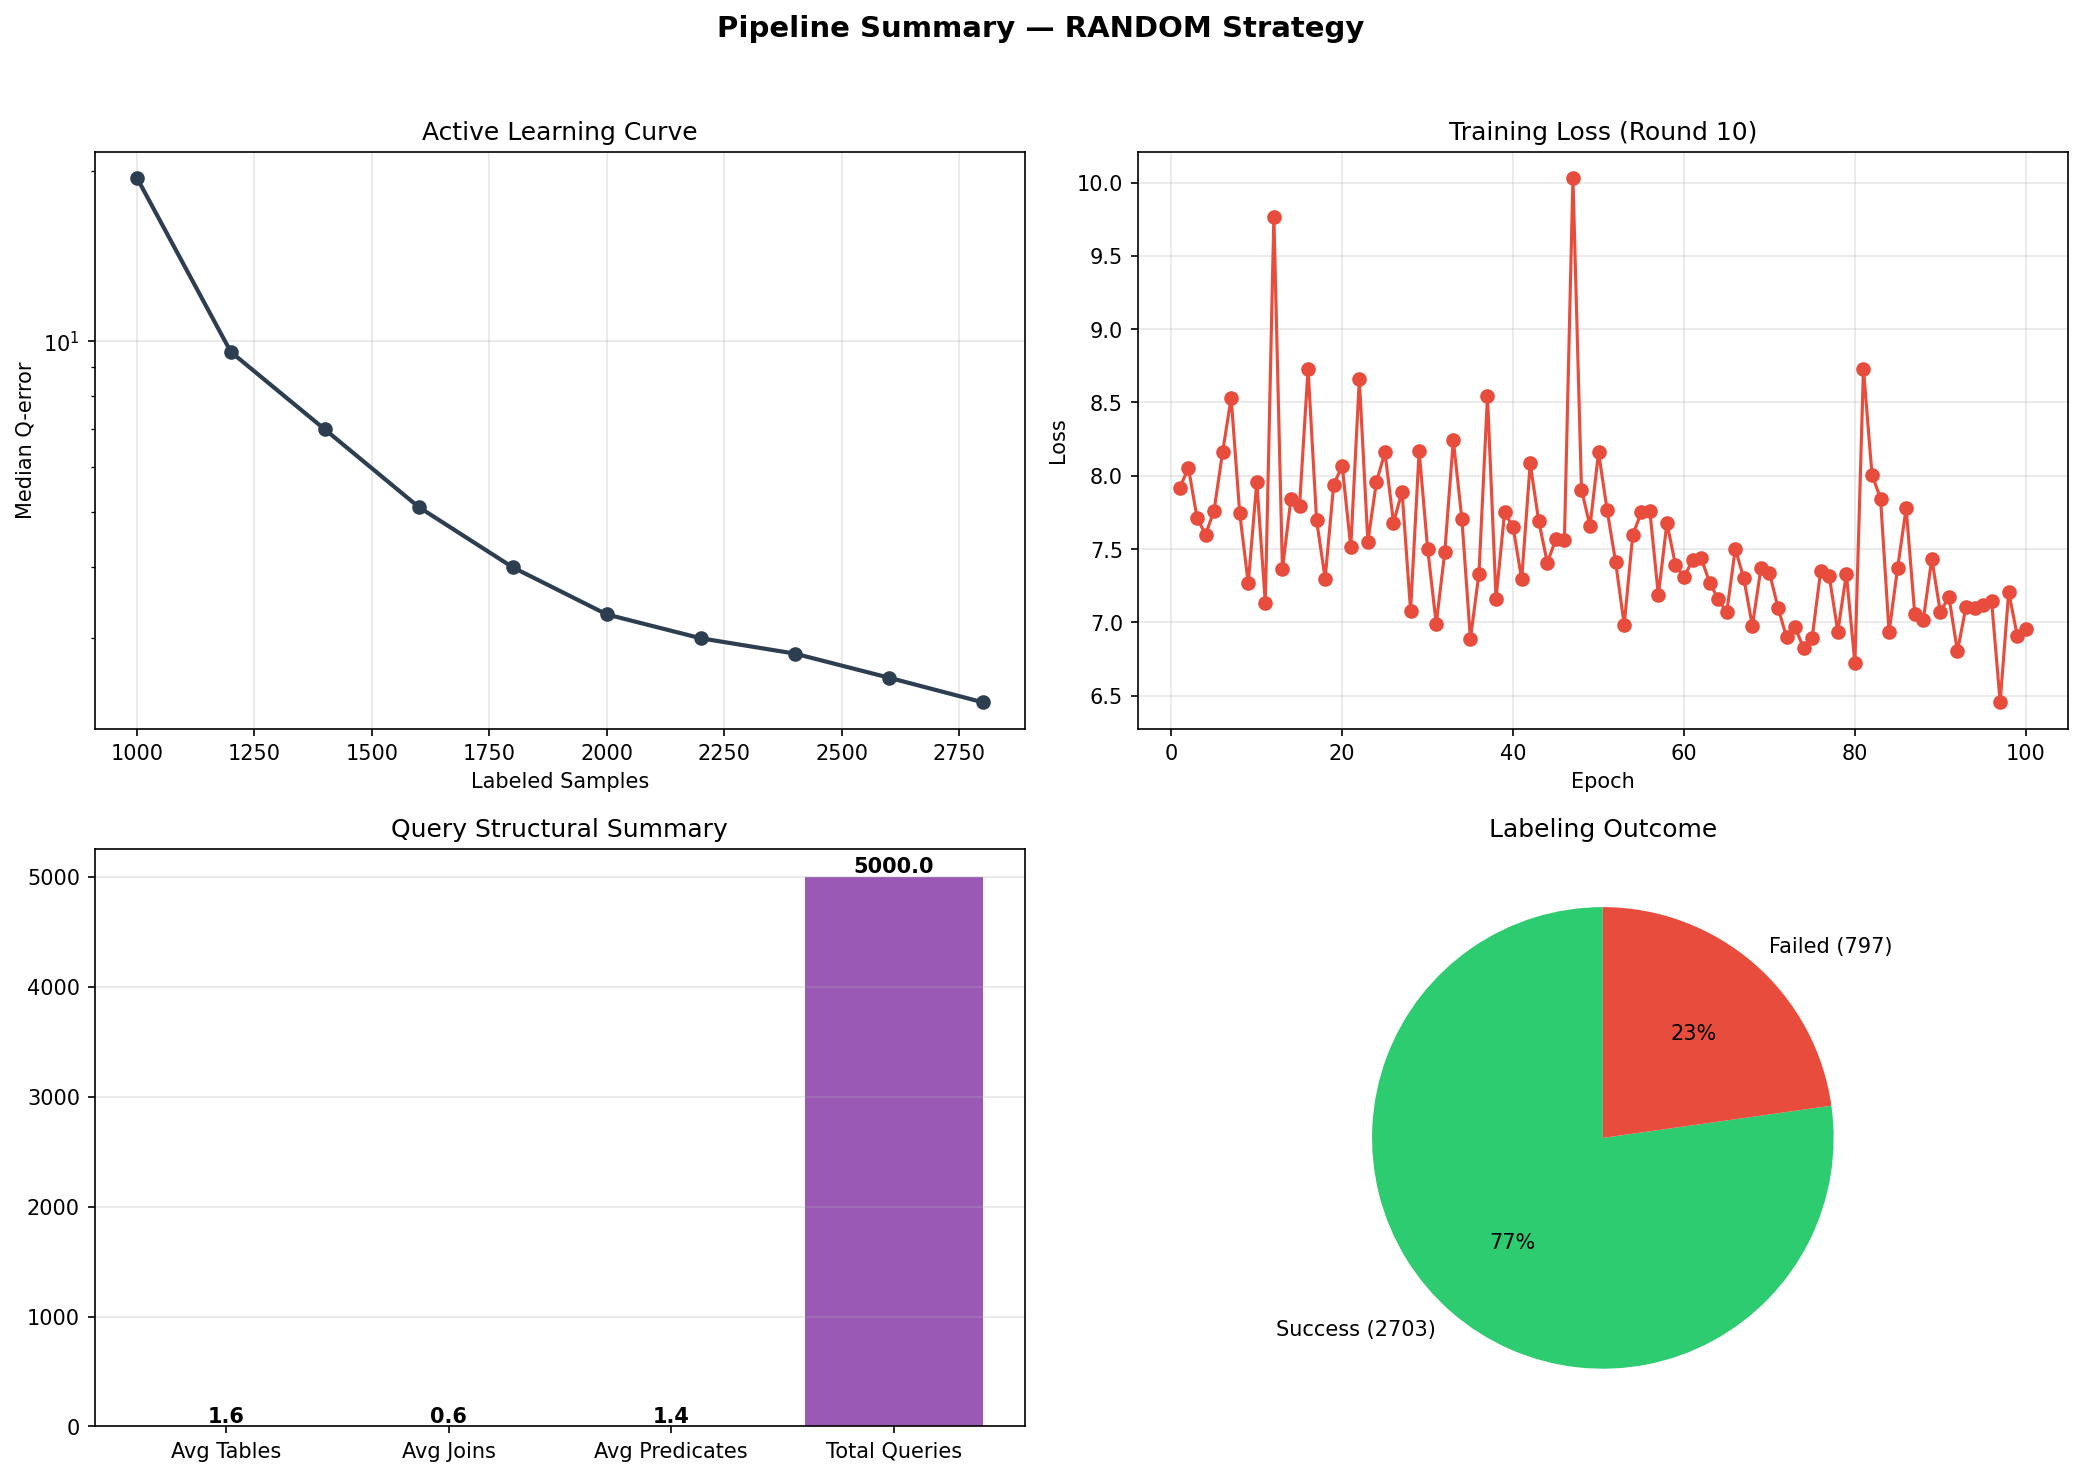
\includegraphics[width=\textwidth]{analysis_pipeline_summary.png}
\caption{Pipeline summary dashboard. Each panel corresponds to a pipeline stage, making it possible to diagnose bottlenecks and quality issues at a glance.}
\label{fig:pipeline_summary}
\end{figure}

A few observations stand out. The validation pipeline rejects only a small fraction of LLM-generated queries, which confirms that the prompt constraints are doing their job. The structural distributions table counts, join counts, predicate counts are well spread rather than clustered around a single pattern, evidence that the diversity hints prevent the LLM from falling into repetitive generation.

The cardinality distribution spans several orders of magnitude, from queries returning a handful of rows to queries returning millions. That breadth is important: a model trained only on mid-range cardinalities would struggle with the extremes, and extremes are precisely where estimation errors cause the most damage to query plans.

The learning curves tell the clearest story about active learning. Accuracy improves with each round, and the improvement is front-loaded the first few rounds contribute the most because the acquisition function targets the low-hanging fruit, the queries that are easiest for the model to learn from. Later rounds bring smaller gains as the remaining unlabeled pool becomes dominated by queries the model already handles reasonably well.

The scatter plots and Q-error distributions confirm that the trained model produces well-calibrated estimates across the full range. Comparing against PostgreSQL's native optimizer puts the learned approach in perspective: the MSCN model, trained on a modest number of labeled queries, can match or beat an optimizer that has access to the full table statistics and histogram infrastructure built into a production database.

Taken together, these results support the central thesis: LLM-based generation combined with active learning is a viable and efficient strategy for training learned cardinality estimators.
